% Marko Ristic

\documentclass[letterpaper, 10 pt, conference]{IEEEtran}

% 
% 8888888 888b     d888 8888888b.   .d88888b.  8888888b. 88888888888 .d8888b.  
%   888   8888b   d8888 888   Y88b d88P" "Y88b 888   Y88b    888    d88P  Y88b 
%   888   88888b.d88888 888    888 888     888 888    888    888    Y88b.      
%   888   888Y88888P888 888   d88P 888     888 888   d88P    888     "Y888b.   
%   888   888 Y888P 888 8888888P"  888     888 8888888P"     888        "Y88b. 
%   888   888  Y8P  888 888        888     888 888 T88b      888          "888 
%   888   888   "   888 888        Y88b. .d88P 888  T88b     888    Y88b  d88P 
% 8888888 888       888 888         "Y88888P"  888   T88b    888     "Y8888P"  
%                                                                              
%                                                                              
%                                                                              
% 

% Graphics
\usepackage{graphicx}
% Maths
\usepackage{amsmath}
\usepackage{amsfonts}
\usepackage{amsthm}
% Local
\usepackage{ISASmacros/isasmathmacros}
% Equal last columns
\usepackage{flushend}
% Fit more per page
%\usepackage{microtype}

% Environments
\theoremstyle{definition}
\newtheorem{definition}{Definition}[section]

% correct bad hyphenation here
\hyphenation{op-tical net-works semi-conduc-tor}

\begin{document}

% paper title
\title{Cryptographically Privileged State Estimation With Gaussian Keystreams}

% author names and affiliations
\author{\IEEEauthorblockN{Marko Ristic}
\IEEEauthorblockA{Intelligent Sensor-Actuator-\\
Systems (ISAS)\\
Karlsruhe Institute of\\
Technology (KIT), Germany\\
Email: marko.ristic@kit.edu}
\and
\IEEEauthorblockN{Benjamin Noack}
\IEEEauthorblockA{Intelligent Sensor-Actuator-\\
Systems (ISAS)\\
Karlsruhe Institute of\\
Technology (KIT), Germany\\
Email: noack@kit.edu}
\and
\IEEEauthorblockN{Uwe D. Hanebeck}
\IEEEauthorblockA{Intelligent Sensor-Actuator-\\
Systems (ISAS)\\
Karlsruhe Institute of\\
Technology (KIT), Germany\\
Email: uwe.hanebeck@kit.edu}}

% make the title area
\maketitle

% 
%        d8888 888888b.    .d8888b. 88888888888 8888888b.         d8888  .d8888b. 88888888888 
%       d88888 888  "88b  d88P  Y88b    888     888   Y88b       d88888 d88P  Y88b    888     
%      d88P888 888  .88P  Y88b.         888     888    888      d88P888 888    888    888     
%     d88P 888 8888888K.   "Y888b.      888     888   d88P     d88P 888 888           888     
%    d88P  888 888  "Y88b     "Y88b.    888     8888888P"     d88P  888 888           888     
%   d88P   888 888    888       "888    888     888 T88b     d88P   888 888    888    888     
%  d8888888888 888   d88P Y88b  d88P    888     888  T88b   d8888888888 Y88b  d88P    888     
% d88P     888 8888888P"   "Y8888P"     888     888   T88b d88P     888  "Y8888P"     888     
%                                                                                             
%                                                                                             
%                                                                                             
% 

\begin{abstract}
State estimation via public channels requires additional planning with regards to state privacy and information leakage of involved parties. In some scenarios, it is desirable to allow partial leakage of state information, thus distinguishing between privileged and unprivileged estimators and their capabilities. In state estimation, existing methods that distinguish between privileged and unprivileged, or trusted and untrusted, estimators typically result in reduced estimation quality for both parties or require additional secure communication channels. We introduce a method to decrease estimation quality at an unprivileged estimator using a stream of pseudorandom Gaussian samples while leaving privileged estimation unaffected and requiring no additional transmission beyond an initial key exchange. First, a cryptographic definition of privileged Bayesian estimation is presented, capturing a definition for the difference between estimations, before a privileged estimation scheme meeting the defined security criteria is developed. Achieving privileged estimation without additional channel requirements allows quantifiable estimation to be made available to the public while keeping the best estimation private to trusted privileged parties and can find uses in a variety of service-providing and privacy-preserving scenarios.
\end{abstract}

% no keywords

% For peer review papers, this IEEEtran command inserts a page break and
% creates the second title. It will be ignored for other modes.
\IEEEpeerreviewmaketitle

% 
% 8888888 888b    888 88888888888 8888888b.   .d88888b.  
%   888   8888b   888     888     888   Y88b d88P" "Y88b 
%   888   88888b  888     888     888    888 888     888 
%   888   888Y88b 888     888     888   d88P 888     888 
%   888   888 Y88b888     888     8888888P"  888     888 
%   888   888  Y88888     888     888 T88b   888     888 
%   888   888   Y8888     888     888  T88b  Y88b. .d88P 
% 8888888 888    Y888     888     888   T88b  "Y88888P"  
%                                                        
%                                                        
%                                                        
% 

\section{Introduction}
% no \IEEEPARstart
The role of state estimation and sensor data processing has become increasingly prevalent in modern systems \cite{ligginsDistributedDataFusion2012}. Particularly, since the development of Kalman estimation theory, Bayesian state estimation has found common application, varying from autonomous systems to remote estimation \cite{mutambaraDecentralizedEstimationControl1998,sinopoliKalmanFilteringIntermittent2004}. As advancements in distributed algorithms and cloud computing develop, the use of wireless and public communication channels for data transmission has become widespread, bringing to light the requirements of data privacy and state secrecy \cite{renSecurityChallengesPublic2012,brennerSecretProgramExecution2011}.

Typically, use-cases for preserving data privacy over public channels involve hiding all transferred information such that eavesdroppers or present untrusted parties learn no additional information from the observed data. This is achievable using common encryption schemes such as AES \cite{gueronIntelAdvancedEncryption2010} or RSA \cite{rivestMethodObtainingDigital1978} which formally capture this security requirement by satisfying cryptographic ciphertext indistinguishability \cite{katzIntroductionModernCryptography2008}. Some more advanced requirements using public channels also exist. When partial information needs to be made public, or computations need to be performed on data, homomorphic or aggregation encryption schemes can be used. \cite{alanwarPrOLocResilientLocalization2017} proposes localization where individual sensors and measurements remain private using homomorphic encryption. \cite{alexandruPrivateWeightedSum2020} has distributed control inputs aggregated without parties learning individual contributions, while \cite{alexandruEncryptedCooperativeControl2019,farokhiSecurePrivateControl2017} use homomorphic encryption to allow control inputs to be computed without decryption. In the context of estimation, a quantifiable difference in estimation performance between untrusted and trusted parties can provide different levels of estimation privilege. This was achieved in the initial release of the Global Positioning System (GPS) \cite{grovesPrinciplesGNSSInertial2015}, which relied on a second, encrypted, stream of information required for accurate estimation. Another example is seen in \cite{leongTransmissionSchedulingRemote2019}, where intermittent sending is proposed to increase eavesdropper estimation error while using a secure feedback channel to ensure better estimation for trusted parties. Our contribution in this work considers this context of privileged and unprivileged estimation and is comprised of a formal definition of privileged Bayesian state estimation, crucial for providing cryptographic security, before proposing an estimation scheme that provides privileged levels of estimation without reliance on additional secure channels or estimator feedback. We accompany the method with a cryptographic proof sketch and simulation results.

In section \ref{sec:problem_statement} we introduce the relevant privileged estimation problem followed by a cryptographic formalisation of desired properties. Section \ref{sec:priv_estimation} introduces our proposed privileged estimation scheme and in section \ref{sec:scheme_security} a cryptographic proof sketch is given. A simulation of the method is then demonstrated and explained in section \ref{sec:simulation}, while concluding remarks and future work are discussed in section \ref{sec:conclusion}.

% 
% ##    ##  #######  ########    ###    ######## ####  #######  ##    ## 
% ###   ## ##     ##    ##      ## ##      ##     ##  ##     ## ###   ## 
% ####  ## ##     ##    ##     ##   ##     ##     ##  ##     ## ####  ## 
% ## ## ## ##     ##    ##    ##     ##    ##     ##  ##     ## ## ## ## 
% ##  #### ##     ##    ##    #########    ##     ##  ##     ## ##  #### 
% ##   ### ##     ##    ##    ##     ##    ##     ##  ##     ## ##   ### 
% ##    ##  #######     ##    ##     ##    ##    ####  #######  ##    ## 
% 

\subsection{Notation}
Throughout this work the following notation is used. Lowercase underlined characters $\vec{a}$ denote vectors, while uppercase bold characters $\mat{M}$ denote matrices. $\mat{M}\succ 0$ and $\mat{M} \succeq 0$ denote positive definitiveness and positive semi-definitiveness, respectively, and $\mat{M} \succ \mat{N}$ is shorthand for $\mat{M}-\mat{N}\succ 0$. Function $\mathsf{eig}(\mat{M})$ gives the set of eigenvalues for matrix $\mat{M}$, $\mathsf{Cov}[\cdot]$ computes the covariance of a random vector, $\mat{I}$ and $\mat{0}$ are the identity and zero matrices, respectively, with size inferrable from context, and $\sim$ denotes distribution while $\dot{\sim}$ denotes pseudorandom distribution.

% 
% 8888888b.  8888888b.   .d88888b.  888888b.   
% 888   Y88b 888   Y88b d88P" "Y88b 888  "88b  
% 888    888 888    888 888     888 888  .88P  
% 888   d88P 888   d88P 888     888 8888888K.  
% 8888888P"  8888888P"  888     888 888  "Y88b 
% 888        888 T88b   888     888 888    888 
% 888        888  T88b  Y88b. .d88P 888   d88P 
% 888        888   T88b  "Y88888P"  8888888P"  
%                                              
%                                              
%                                              
% 

\section{Problem Statement}\label{sec:problem_statement}
We consider the estimation scenario where process and measurement models are known and stochastic, and state estimators are either privileged possessing a secret key or unprivileged without. We aim to develop a scheme for which the difference in their estimation errors is quantifiable and cryptographically guaranteed when process and measurement models are Gaussian, linear, and time-invariant.

The process model we consider gives the state $\vec{x}_k\in\mathbb{R}^n$ at an integer timestep $k$ and is given by
\begin{equation}\label{eqn:linear_process_model}
   \vec{x}_k = \mat{F}\vec{x}_{k-1} + \vec{w}_k\,,
\end{equation}
with noise term $\vec{w}_k\sim \mathcal{N}(\vec{0}, \mat{Q})$ and a known non-zero covariance $\mat{Q}\in \mathbb{R}^{n\times n}$. Similarly, the measurement model gives the measurement $\vec{y}_k$ at a time $k$ and is given by
\begin{equation}\label{eqn:linear_measurement_model}
   \vec{y}_k = \mat{H}\vec{x}_k + \vec{v}_k\,,
\end{equation}
with noise term $\vec{v}_k\sim \mathcal{N}(\vec{0}, \mat{R})$ and a known non-zero covariance $\mat{R}\in \mathbb{R}^{m\times m}$.

To capture our aim of creating a privileged and unprivileged estimator, we must first define how to assess the estimation advantage between estimators, and which algorithms are required to characterize a privileged estimation scheme. In the following section, we give relevant formal definitions, which will be used when assessing the security of our proposed scheme.

% 
%  ######  ########  ##    ## ########  ########  #######  
% ##    ## ##     ##  ##  ##  ##     ##    ##    ##     ## 
% ##       ##     ##   ####   ##     ##    ##    ##     ## 
% ##       ########     ##    ########     ##    ##     ## 
% ##       ##   ##      ##    ##           ##    ##     ## 
% ##    ## ##    ##     ##    ##           ##    ##     ## 
%  ######  ##     ##    ##    ##           ##     #######  
% 

\subsection{Formal cryptographic Problem}\label{subsec:crypto_problem}
While we are interested in Gaussian, linear, and time-invariant models, it is more practical to define a broader security notion that can be satisfied under arbitrary specified conditions on the models. This allows the use of the security notion in future literature and is more in-line with typical cryptographic practice. We will later show that our proposed scheme meets this security notion under the specific Gaussian, linear and time-invariant model assumptions.

Typical formal cryptographic security notions are given in terms of probabilistic polynomial-time (PPT) attackers and capture desired privacy properties as well as attacker capabilities \cite{katzIntroductionModernCryptography2008}. The most commonly desired privacy property, cryptographic indistinguishability, is not suitable for our estimation scenario due to our desire for unprivileged estimators to gain \text{some} information from measurements. Instead, we will define security in terms of a time series of covariances, given arbitrary known models, such that the difference in estimation error between estimators with and without the secret key is bounded by the series at all times.

To formalize this, we introduce the following notations and definitions. We assume the existence of an arbitrary process (not necessarily Gaussian or linear) following a known model exactly, with the state at time $k$ denoted $\vec{x}_k\in\mathbb{R}^n$ and model parameters $\mathcal{M}_P$. Similarly, we assume the existence of a means of process measurement following a known measurement model exactly, with the measurement at time $k$ denoted $\vec{y}_k\in\mathbb{R}^m$ and model parameters $\mathcal{M}_M$. We can now define a \textit{privileged estimation scheme} as a pair of algorithms $(\mathsf{Setup},\mathsf{Noise})$ given by
\begin{LaTeXdescription}
   \item[$\mathsf{Setup}(\mathcal{M}_P, \mathcal{M}_M, \kappa)$] On the input of models $\mathcal{M}_P$ and $\mathcal{M}_M$, and the security parameter $\kappa$, public parameters $\mathsf{pub}$ and a secret key $\mathsf{sk}$ are created.
   \item[$\mathsf{Noise}(\mathsf{sk}, k, \mathcal{M}_P, \mathcal{M}_M, \vec{y}_1, \dots, \vec{y}_k)$] On input of secret key $\mathsf{sk}$, time $k$, models $\mathcal{M}_P$ and $\mathcal{M}_M$, and measaurements $y_1,\dots,y_k$, a noisy measurement $\vec{y}^\prime_k$ (with no required model constraints) is created.
\end{LaTeXdescription}
In addition to the scheme description above, we also give the following definitions to help formalize our desired security notion.
\begin{definition}\label{def:estimator}
   An \textit{estimator} is any probabilistic algorithm that produces a guess of the state $\vec{x}_k$ for a given time $k$.
\end{definition}
\begin{definition}
   A \textit{negligible covariance function} is a function 
   \begin{equation}
      \mathsf{neglCov}_m(\kappa):\mathbb{N}\rightarrow \mathbb{R}^{m\times m}
   \end{equation}
   that returns a matrix $\mat{A}$ such that $\mat{A}$ is a valid covariance ($\mat{A}\succ 0$ and $\mat{A}=\mat{A}^\top$) and that for each of its eigenvalues $e\in\mathsf{eig}(\mat{A})$, there exists a negligible function $\eta$ such that $e\leq\eta(\kappa)$.
\end{definition}

With the terminology above, we can now introduce the security notion which captures the formal requirements of the estimation problem that we want to solve.
\begin{definition}\label{def:cov_privilege_security_notion}
   A privileged estimation scheme meets notion \textit{$\{\mat{D}_1,\mat{D}_2,\dots\}$-Covariance Privilege for Models $\mathcal{M}_P$ and $\mathcal{M}_M$} if for any PPT estimator $\mathcal{A}$, there exists a PPT estimator $\mathcal{A}^\prime$, such that
   \begin{equation}\label{eqn:cov_privilege}
      \begin{split}
         &\mathsf{Cov}\left[\mathcal{A}\left(k, \kappa, \mathsf{pub}, \mathcal{M}_P, \mathcal{M}_M, \vec{y}^\prime_1,\dots,\vec{y}^\prime_k\right) - \vec{x}_k \right]\\
         &-\mathsf{Cov}\left[\mathcal{A}^\prime\left(k, \kappa, \mathsf{pub}, \mathcal{M}_P, \mathcal{M}_M, \vec{y}_1,\dots,\vec{y}_k\right) - \vec{x}_k \right]\\
         &\quad\succeq \mat{D}_k + \mathsf{neglCov}_m(\kappa)
      \end{split}
   \end{equation}
   for valid covariances $\mat{D}_k$ and some negligible covariance function for all $k>0$. Here, estimators $\mathcal{A}$ and $\mathcal{A}^\prime$ are running in polynomial-time with respect to the security parameter $\kappa$, and all probabilities are taken over models $\mathcal{M}_P$ and $\mathcal{M}_M$, estimators $\mathcal{A}$ and $\mathcal{A}^\prime$, and algorithms $\mathsf{Setup}$ and $\mathsf{Noise}$.
\end{definition}

Informally, the above definition states that no estimator that can only access noisy measurements $\vec{y}^\prime_1,\dots,\vec{y}^\prime_k$ can estimate a state $\vec{x}_k$ for a time $k$ with a mean square error (MSE) covariance less than an equivalent estimator with access to true measurements $\vec{y}_1,\dots,\vec{y}_k$, by a margin of at least $\mat{D}_k$. We also note that by taking probabilities over the process model, and therefore the true states $\vec{x}_k$, the definition is Bayesian for any stochastic process model. Next, we will propose a scheme meeting the aforementioned notion for a derivable series of covariances when models $\mathcal{M}_P$ and $\mathcal{M}_M$ are Gaussian, linear, and time-invariant.

% 
% 8888888b.  8888888b.  8888888 888     888      8888888888 .d8888b. 88888888888 
% 888   Y88b 888   Y88b   888   888     888      888       d88P  Y88b    888     
% 888    888 888    888   888   888     888      888       Y88b.         888     
% 888   d88P 888   d88P   888   Y88b   d88P      8888888    "Y888b.      888     
% 8888888P"  8888888P"    888    Y88b d88P       888           "Y88b.    888     
% 888        888 T88b     888     Y88o88P        888             "888    888     
% 888        888  T88b    888      Y888P         888       Y88b  d88P    888     
% 888        888   T88b 8888888     Y8P          8888888888 "Y8888P"     888     
%                                                                                
%                                                                                
%                                                                                
% 

\section{Privileged Estimation}\label{sec:priv_estimation}
The general idea behind our privileged estimation scheme is adding pseudorandom noise to measurements at the sensor, degrading the state estimation at estimators that cannot remove it. The added noise is a keystream generated from a secret key and can be generated and removed from measurements by any sensor holding the same key.

To allow meeting the cryptographic notion in section \ref{subsec:crypto_problem} we focus on Gaussian, linear and time-invariant models where the minimum achievable error covariance is easily computable, and produce a keystream of pseudorandom Gaussian noise. The keystream and added noise are given next.

% 
% ##    ## ######## ##    ##  ######  ######## ########  ########    ###    ##     ## 
% ##   ##  ##        ##  ##  ##    ##    ##    ##     ## ##         ## ##   ###   ### 
% ##  ##   ##         ####   ##          ##    ##     ## ##        ##   ##  #### #### 
% #####    ######      ##     ######     ##    ########  ######   ##     ## ## ### ## 
% ##  ##   ##          ##          ##    ##    ##   ##   ##       ######### ##     ## 
% ##   ##  ##          ##    ##    ##    ##    ##    ##  ##       ##     ## ##     ## 
% ##    ## ########    ##     ######     ##    ##     ## ######## ##     ## ##     ## 
% 

\subsection{Gaussian Keystream}\label{subsec:gaussian_keystream}
To generate pseudorandom Gaussian samples, we rely on first generating a typical cryptographic pseudorandom bitstream given a secret key $\mathsf{sk}$. Using a well-studied method for the generation of pseudorandomness guarantees robustness and easy updating should a used scheme no longer be considered safe. Any cryptographic stream cipher can be used and we interpret the bitstream as sequential pseudorandom integers $q_t \in \mathbb{N}$, of a suitable size, for integer indexes $t>0$ and use them to generate a sequence of pseudorandom uniform real numbers $u_t\ \dot{\sim}\ \mathcal{U}(0,1)$.

The conversion of $q_t$ to $u_t$ is cryptographically non-trivial due to the floating-point representation of $u_t$. Since it cannot be truly representative of the distribution $\mathcal{U}(0,1)$, the pseudorandomness of samples is affected, and meeting the desired cryptographic notion is complicated. For now, we will assume that the uniform floating-point numbers (floats) are sufficiently close to true uniform reals, as is the current industry standard, and rely on any common method for choosing the bit size of integers $q_t$ and the pseudorandom generation of uniforms $u_t$ \cite{goualardGeneratingRandomFloatingPoint2020}. In section \ref{sec:scheme_security} we will state and further discuss this assumption.

Given the sufficiently uniform pseudorandom floats $u_t$, we are left with generating a series of pseudorandom standard normal Gaussian samples, which can be readily computed using the Box-Muller transform \cite{paleyFourierTransformsComplex1934}, by
\begin{equation}
   z_t = \sqrt{-2\ln (u_t)}\cos(2\pi u_{t+1})
\end{equation}
and
\begin{equation}
   z_{t+1} = \sqrt{-2\ln (u_t)}\sin(2\pi u_{t+1})
\end{equation}
to obtain two sequential, independent, standard normal Gaussian samples from two uniform ones. This Gaussian keystream can then be used by a privileged estimation scheme to add arbitrary pseudorandom multivariate Gaussian noises.

% 
%    ###    ########  ########     ##    ##  #######  ####  ######  ######## 
%   ## ##   ##     ## ##     ##    ###   ## ##     ##  ##  ##    ## ##       
%  ##   ##  ##     ## ##     ##    ####  ## ##     ##  ##  ##       ##       
% ##     ## ##     ## ##     ##    ## ## ## ##     ##  ##   ######  ######   
% ######### ##     ## ##     ##    ##  #### ##     ##  ##        ## ##       
% ##     ## ##     ## ##     ##    ##   ### ##     ##  ##  ##    ## ##       
% ##     ## ########  ########     ##    ##  #######  ####  ######  ######## 
% 

\subsection{Additional Gaussian Noise}\label{subsec:adding_privilege_noise}
To use the series of pseudorandom Gaussian samples $z_t$, $t>0$, at the sensor and privileged estimator, they need to be converted to $n$-dimension zero-mean multivariate Gaussian samples suitable for use in the measurement model \eqref{eqn:linear_measurement_model}, at every time $k$. In addition, we want control over the difference in estimation error between privileged and unprivileged estimators, and do so by including the symettric matrix parameter $\mat{Z}\succ 0$, in a way that added pseudorandom noise $\vec{p}_k$ at time $k$ is such that $\vec{p}_k\ \dot{\sim}\ \mathcal{N}(\vec{0},\mat{Z})$. Given $\mat{Z}$, $\vec{p}_k$ is computed using the next $n$ Gaussian keystream samples, that is $(k-1)n+1\leq t\leq kn$, as
\begin{equation}
   \vec{p}_k = \mat{Z}\cdot
   \begin{bmatrix}
      z_{(k-1)n+1} & \dots & z_{kn}
   \end{bmatrix}^\top\,.
\end{equation}

Before estimation, we assume that the secret key $\mathsf{sk}$, required for generating the Gaussian keystream in section \ref{subsec:gaussian_keystream}, has been shared between the sensor and privileged estimator. During estimation, the sensor modifies its measurements $\vec{y}_k$ by
\begin{equation}\label{eqn:modified_measurement}
   \vec{y}^\prime_k = \vec{y}_k + \vec{p}_k\,,
\end{equation}
resulting in a new measurement model
\begin{equation}
   \vec{y}^\prime_k = \mat{H}\vec{x}_k + \vec{v}_k + \vec{p}_k\,,
\end{equation}
with $\vec{v}_k\sim \mathcal{N}(\vec{0},\mat{R})$ and $\vec{p}_k\ \dot{\sim}\ \mathcal{N}(\vec{0},\mat{Z})$. There are now two estimation problems present for the privileged and unprivileged estimator respectively.
\begin{LaTeXdescription}
   \item[Privileged estimation] The estimator that holds the secret key $\mathsf{sk}$ can compute the Gaussian key stream $z_t$, $0<t$, and therefore the added noise vectors $\vec{p}_k$ at every time $k$ as well. Computing $\vec{y}_k = \vec{y}^\prime_k - \vec{p}_k$ given the noisy measurements results in the original measurements following measurement model \eqref{eqn:linear_measurement_model} exactly.
   \item[Unprivileged estimation] In the case where pseudorandomness is indistinguishable from randomness, as is the case at an unprivileged estimator when using a cryptographically secure keystream and $\mathsf{sk}$ is not known, noisy measurements are indistinguishable from those following the unprivileged measurement model 
   \begin{equation}\label{eqn:unprivileged_measurement_model}
      \vec{y}^\prime_k = \mat{H}\vec{x}_k + \vec{v}^\prime_k\,,
   \end{equation}
   with $\vec{v}^\prime_k\sim \mathcal{N}(\vec{0},\mat{R}+\mat{Z})$, exactly.
\end{LaTeXdescription}

Intuitively, we can see that the two estimators will have their difference in estimation error dependent on matrix $\mat{Z}$. In the security section, we will show that the best possible error covariances achievable by the privileged and unprivileged estimators can be computed exactly for both measurement models and that the difference between them will give the series $\mat{D}_k$, $k>0$, required for the security notion \eqref{eqn:cov_privilege}.

% 
% ##     ## ##     ## ##       ########    ########  ########  #### ##     ## 
% ###   ### ##     ## ##          ##       ##     ## ##     ##  ##  ##     ## 
% #### #### ##     ## ##          ##       ##     ## ##     ##  ##  ##     ## 
% ## ### ## ##     ## ##          ##       ########  ########   ##  ##     ## 
% ##     ## ##     ## ##          ##       ##        ##   ##    ##   ##   ##  
% ##     ## ##     ## ##          ##       ##        ##    ##   ##    ## ##   
% ##     ##  #######  ########    ##       ##        ##     ## ####    ###    
% 

\subsection{Multiple Privileges}\label{subsec:mult_privileges}
In the above scenario, we have considered a single level of estimation privileged with one private key, dividing estimation error covariance into two groups. As a direct extension, it may be desirable to define multiple \textit{levels} of privilege, such that the best estimation performance depends on the privilege level of an estimator. Here we will briefly put forward one such example, where a single secret key corresponds to each privilege level and noise is added similarly to \eqref{eqn:modified_measurement} for each key individually.

We now have $N$ secret keys $\mathsf{sk}_i$ and covariances for the added noises $\mat{Z}_i$, $1\leq i \leq N$. Sensor measurements are modified by
\begin{equation}\label{eqn:mult_modified_measurement}
   \vec{y}_k^{\prime\prime} = \vec{y}_k + \vec{p}^{(1)}_k + \cdots + \vec{p}^{(N)}_k\,,
\end{equation}
with $\vec{p}^{(i)}_k\ \dot{\sim}\ \mathcal{N}(\vec{0}, \mat{Z}_i)$, $1\leq i \leq N$. From \eqref{eqn:mult_modified_measurement}, we see that obtaining any single key $\mathsf{sk}_i$ leads to a measurement model where only a single pseudorandom Gaussian sample, of covariance $Z_i$, is removed, resulting in measurements indistinguishable from those following the unprivileged measurement model
\begin{equation}
   \vec{y}_k^{(i)} = \mat{H}\vec{x}_k + \vec{v}^{(i)}_k\,,
\end{equation}
where $\vec{v}_k\sim \mathcal{N}(\vec{0},\mat{R}+\mat{E}_i)$, with
\begin{equation}\label{eqn:mult_privilege_covariances}
   \mat{E}_i = \sum^N_{j=1,j \neq i}\mat{Z}_j\,.
\end{equation}
As values $\mat{E}_i$ directly correspond to the relative estimation performances of each privilege level, we are also interested in the numerical restrictions when choosing these matrices. For the models to be valid for any measurement covariance $\mat{R}$, it is clear that $\mat{E}_i\succ 0$ and $\mat{E}=\mat{E}^\top$ must hold for all $1\leq i\leq N$, but due to the dependence of $\mat{Z}_i$ there is an additional restriction required to ensure all values of $\mat{Z}_i$ remain valid covariances as well. From \eqref{eqn:mult_privilege_covariances} we can write
\begin{equation}
   \begin{bmatrix}
      \mat{0} & \mat{I} & \mat{I} & \cdots & \mat{I}\\
      \mat{I} & \mat{0} & \mat{I} & \cdots & \mat{I}\\
      \vdots & \ddots & \ddots & \ddots & \vdots\\
      \mat{I} & \cdots & \mat{I} & \mat{0} & \mat{I}\\
      \mat{I} & \cdots & \mat{I} & \mat{I} & \mat{0}
   \end{bmatrix}
   \begin{bmatrix}
      \mat{Z}_1\\
      \mat{Z}_2\\
      \vdots\\
      \mat{Z}_{N-1}\\
      \mat{Z}_N
   \end{bmatrix}
   =
   \begin{bmatrix}
      \mat{E}_1\\
      \mat{E}_2\\
      \vdots\\
      \mat{E}_{N-1}\\
      \mat{E}_N
   \end{bmatrix}\,,
\end{equation}
which, when rearranged and the conditions $\mat{Z}_i\succ 0$ are taken into account, gives the additional requirement
\begin{equation}\label{eqn:mult_covariance_restriction}
   \mat{E}_i \prec \frac{1}{N-1}\sum_{j=1}^{N}\mat{E}_j
\end{equation}
for all $1 \leq i \leq N$.

From \eqref{eqn:mult_covariance_restriction} we can see that privilege levels are significantly restricted in relative estimation performance. We have demonstrated this method due to its simplicity and relation to the single-level scheme, however, alternative methods involving multiple or overlapping keys may allow weaker restrictions and will be considered in future work.

% 
%  .d8888b.  8888888888 .d8888b.  888     888 8888888b.  8888888 88888888888 Y88b   d88P 
% d88P  Y88b 888       d88P  Y88b 888     888 888   Y88b   888       888      Y88b d88P  
% Y88b.      888       888    888 888     888 888    888   888       888       Y88o88P   
%  "Y888b.   8888888   888        888     888 888   d88P   888       888        Y888P    
%     "Y88b. 888       888        888     888 8888888P"    888       888         888     
%       "888 888       888    888 888     888 888 T88b     888       888         888     
% Y88b  d88P 888       Y88b  d88P Y88b. .d88P 888  T88b    888       888         888     
%  "Y8888P"  8888888888 "Y8888P"   "Y88888P"  888   T88b 8888888     888         888     
%                                                                                        
%                                                                                        
%                                                                                        
% 

\section{Scheme Security}\label{sec:scheme_security}
The security of the proposed scheme will be primarily considered in the single privileged estimation level as introduced in section \ref{subsec:adding_privilege_noise} and a proof sketch will be provided to show how the proposed scheme meets the cryptographic notion \eqref{eqn:cov_privilege}. The extension to multiple privilege levels as described in section \ref{subsec:mult_privileges} will be informally discussed afterward.

% 
%  ######  #### ##    ##  ######   ##       ######## 
% ##    ##  ##  ###   ## ##    ##  ##       ##       
% ##        ##  ####  ## ##        ##       ##       
%  ######   ##  ## ## ## ##   #### ##       ######   
%       ##  ##  ##  #### ##    ##  ##       ##       
% ##    ##  ##  ##   ### ##    ##  ##       ##       
%  ######  #### ##    ##  ######   ######## ######## 
% 

\subsection{Single Privileged Case}
Recalling the security notion in section \eqref{eqn:linear_measurement_model}, we now aim to show how our single privilege level estimation scheme in section \ref{subsec:adding_privilege_noise}, given conditions on $\mathcal{M}_P$ and $\mathcal{M}_M$, meets the notion for a computable series $\mat{D}_k$, $k>0$, dependent on the noise parameter $\mat{Z}$.

We consider the Bayesian process model \eqref{eqn:linear_process_model} and measurement model \eqref{eqn:linear_measurement_model} exactly, that is, any time-invariant linear models with known zero-mean Gaussian additive noises. We define these are our model conditions and capture all relevant parameters from the respective equations in $\mathcal{M}_P$ and $\mathcal{M}_M$. Our scheme fulfills the two required algorithms for a privileged estimation scheme, $\mathsf{Setup}$ and $\mathsf{Noise}$, as follows.
\begin{LaTeXdescription}
   \item[$\mathsf{Setup}$] Initialise a cryptographically indistinguishable stream cipher with the parameter $\kappa$, set the secret key $\mathsf{sk}$ to the stream cipher key and include an initial filter estimate $\hat{\vec{x}}_0$, error covariance $\mat{P}_0$ and added noise variance $\mat{Z}$ in the public parameters $\mathsf{pub}$.
   \item[$\mathsf{Noise}$] Computed by \eqref{eqn:modified_measurement}, returning $\vec{y}^\prime_k$ as the noisy measurement at time $k$, with added pseudorandom Gaussian noise computed from the stream cipher using $\mathsf{sk}$.
\end{LaTeXdescription}
Additionally, we note that in the above $\mathsf{Setup}$ algorithm, the inclusion of the initial state and added noise covariance are not a requirement for the security of the scheme, but merely make relevant estimation parameters public for completeness.

The idea behind our security roof relies on the optimality of the linear Kalman Filter (KF) \cite{haugBayesianEstimationTracking}. Given an initial estimate and estimate error covariance, the KF produces posterior Bayesian estimates with the minimum mean square error (MSE) achievable for \textit{any} estimator when all measurements $\vec{y}_1,\dots,\vec{y}_k$ are observed, models are Gaussian and linear, and the same initialization is used. Since the KF also preserves initial error covariance order,
\begin{equation}
   \mat{P}_k \preceq \mat{P}_k^\prime \implies \mat{P}_{k+1} \preceq \mat{P}_{k+1}^\prime\,,
\end{equation}
we can define an error covariance lower-bound $\mat{P}_k^{(l)}$ for all possible initialisations by setting $\mat{P}_0^{(l)} = \mat{0}$ and computing the posterior KF error covariance using the combined predict and update equations
\begin{equation}\label{eqn:lower_bound_error_cov}
   \begin{split}
      \mat{P}_k^{(l)} =& \Bigl( \mat{I} - (\mat{F}\mat{P}_{k-1}^{(l)}\mat{F}^\top + \mat{Q})\mat{H}^\top \cdot \\
      &\qquad(\mat{H}(\mat{F}\mat{P}_{k-1}^{(l)}\mat{F}^\top + \mat{Q})\mat{H}^\top + \mat{R})^{-1}\mat{H}\Bigr)\cdot\\
      &\Bigl(\mat{F}\mat{P}_{k-1}^{(l)}\mat{F}^\top + \mat{Q}\Bigr)\,.
   \end{split}
\end{equation}
This gives us a lower-bound at every time $k$, such that
\begin{equation}
   \mat{P}_k^{(l)} \preceq \mathsf{Cov}\left[\mathcal{A}\left(k, \mathcal{M}_P, \mathcal{M}_M, \vec{y}_1,\dots,\vec{y}_k\right) - \vec{x}_k \right]
\end{equation}
for any estimator $\mathcal{A}$ following definition \ref{def:estimator} and any Gaussian, linear and time-invariant models $\mathcal{M}_P$ and $\mathcal{M}_M$. This leads us into the sketch proof.

\subsubsection{Proof Sketch}
As a cryptographically pseudorandom stream cipher is used in section \ref{subsec:gaussian_keystream}, the stream integers $q_t$, and therefore the uniform samples $u_t$ and normal Gaussian samples $z_t$, are indistinguishable to those generated from a truly random stream for any PPT estimator without the secret key. We persist with the previous assumption that floating-point representations of $z_t$ are sufficiently close to Gaussian and assume the KF to provide optimal estimation when using floats, as is standard in the state-of-the-art. Using the $\mathsf{Setup}$ and $\mathsf{Noise}$ algorithms for our scheme now leads to pseudorandom noisy measurements $\vec{y}^\prime_k$ that are indistinguishable from measurements following the unprivileged measurement model \eqref{eqn:unprivileged_measurement_model}. We can now compute a lower-bound $\mat{P}_k^{\prime(l)}$ for any unprivileged estimator as $\mat{P}_k^{\prime(l)}=\mat{0}$ and
\begin{equation}\label{eqn:unprivileged_lower_bound_error_cov}
   \begin{split}
      \mat{P}_k^{\prime(l)} =& \Bigl( \mat{I} - (\mat{F}\mat{P}_{k-1}^{\prime(l)}\mat{F}^\top + \mat{Q})\mat{H}^\top \cdot \\
      &\qquad(\mat{H}(\mat{F}\mat{P}_{k-1}^{\prime(l)}\mat{F}^\top + \mat{Q})\mat{H}^\top + \mat{R}+\mat{Z})^{-1}\mat{H}\Bigr)\cdot\\
      &\Bigl(\mat{F}\mat{P}_{k-1}^{\prime(l)}\mat{F}^\top + \mat{Q}\Bigr)\,.
   \end{split}
\end{equation}
Taking the difference of bounds \eqref{eqn:unprivileged_lower_bound_error_cov} and \eqref{eqn:lower_bound_error_cov} produces the series
\begin{equation}\label{eqn:covariance_difference_series}
   \mat{D}_k = \mat{P}_k^{\prime(l)} - \mat{P}_k^{(l)}\,,
\end{equation}
for $k>0$, which can be scaled by the parameter $\mat{Z}$. Since both series $\mat{P}_k^{(l)}$ and $\mat{P}_k^{\prime(l)}$ give the lowest possible error covariance of the respective estimators, an estimator following model \eqref{eqn:linear_measurement_model} can always be created for one following the model \eqref{eqn:unprivileged_measurement_model} such that their error covariances at any time $k$ differ by at least $\mat{D}_k$. A reduction proof can be easily constructed where the existence of an unprivileged estimator in our scheme that can produce estimates such that \eqref{eqn:cov_privilege} does not hold, can be used to construct an estimator with an error covariance lower than $\mat{P}_k^{\prime(l)}$ given a known model of the form \eqref{eqn:unprivileged_measurement_model}. As no such estimator exists, we conclude that our scheme meets $\{\mat{D}_1,\mat{D}_2,\dots\}$-Covariance Privilege for Models $\mathcal{M}_P$ and $\mathcal{M}_M$, when $\mathcal{M}_P$ and $\mathcal{M}_M$ are Gaussian, linear and time-invariant. This concludes our proof sketch.

In addition to the proof sketch, we stress caution when accepting a cryptographic guarantee in terms of models $\mathcal{M}_P$ and $\mathcal{M}_M$ when used to estimate a measured physical process or approximate continuous quantities. The following assumptions are made in this scenario.
\begin{LaTeXdescription}
   \item[Exact models] When assigning a model to a physical process, any cryptographic guarantees concerning the model assumes the process follows the model \textit{exactly}. It is often the case that models assume a Bayesian interpretation of probability (a stochastic state) or are chosen to simplify estimation, resulting in the possibility of better estimation given alternative or more complicated models. Although the standard for state estimation, we state the assumption to highlight the distinction between models and a physical process.
   \item[Floating-point approximation] As stated in section \ref{subsec:gaussian_keystream} and the proof sketch above, floating-point approximations to real numbers complicate cryptographic guarantees when relying on mathematical proofs using real numbers such as KF optimality. While optimal estimation with floats is beyond the scope of this work, the prevalence of floats in decades of state estimation justifies the assumption of sufficient similarity and the insignificance of associated error introduced to the security notion.
\end{LaTeXdescription}

% 
% ##     ## ##     ## ##       ######## 
% ###   ### ##     ## ##          ##    
% #### #### ##     ## ##          ##    
% ## ### ## ##     ## ##          ##    
% ##     ## ##     ## ##          ##    
% ##     ## ##     ## ##          ##    
% ##     ##  #######  ########    ##    
% 

\subsection{Multiple Additional Noises}
We have not defined a security notion for multiple levels of privileged estimation, but an intuitive and informal extension is briefly described here. 

A suitable notion would require that for any subset of corrupted estimators, and thus estimators with any subset of secret keys $S \subseteq \{\mathsf{sk}_i,\,1\leq i\leq N\}$, who are given noisy measurements $\vec{y}_k^{\prime\prime}$, an estimator given true measurements $\vec{y}_k$ can be constructed such that the difference between the corrupted subset's error covariance and its own is at least $\mat{D}^{(S)}_k$ at time $k$. Although this definition requires a series $\mat{D}^{(S)}_k$ for every possible subset of privilege level keys, $S$, complicating its formal specification, it captures the exact advantage of every such subset producing a general definition.

Given the structure of our scheme in section \ref{subsec:mult_privileges} it can be readily seen how the above notion would be met. Similarly to the single level case, the KF can be used to compute the minimum error covariances for all compromised key subsets as well as for an estimator with the true measurements, and the relevant difference series $\mat{D}^{(S)}_k$ can be defined. 

% 
%  .d8888b. 8888888 888b     d888 
% d88P  Y88b  888   8888b   d8888 
% Y88b.       888   88888b.d88888 
%  "Y888b.    888   888Y88888P888 
%     "Y88b.  888   888 Y888P 888 
%       "888  888   888  Y8P  888 
% Y88b  d88P  888   888   "   888 
%  "Y8888P" 8888888 888       888 
%                                 
%                                 
%                                 
% 

\section{Simulation and Results}\label{sec:simulation}
As well as showing the theoretical security of our scheme, we have simulated the Bayesian estimation problem using linear Kalman filter estimators for the different measurement models. Simulations have been implemented in the Python programming language and use the AES block cipher in CTR mode as a cryptographically secure stream cipher (AES-CTR) \cite{gueronIntelAdvancedEncryption2010}.

We have considered two simulations, both following the same two-dimensional constant-velocity process model, given by
\begin{equation*}
   \mat{F}=
   \begin{bmatrix}
      1 & 0.5 & 0 & 0\\
      0 & 1 & 0 & 0\\
      0 & 0 & 1 & 0.5\\
      0 & 0 & 0 & 1
   \end{bmatrix}
\end{equation*}
and
\begin{equation*}
   \mat{Q}=0.01\cdot
   \begin{bmatrix}
      0.0417 & 0.1250 & 0 & 0\\
      0.1250 & 0.5000 & 0 & 0\\
      0 & 0 & 0.0417 & 0.1250\\
      0 & 0 & 0.1250 & 0.5000
   \end{bmatrix}\,,
\end{equation*}
with differing measurement models. In all cases, estimators were initialized with the same initial conditions, equal to the true starting condition of the processes they were estimating with initial error covariance $\mat{0}$.

The first measurement model measures location and leads to an observable system with bounded error covariances as $k \rightarrow \infty$. It is given by
\begin{equation*}\label{eqn:bounded_sim_measurement_model}
   \mat{H}=
   \begin{bmatrix}
      1 & 0 & 0 & 0\\
      0 & 0 & 1 & 0
   \end{bmatrix}
   \text{ and }
   \mat{R}=
   \begin{bmatrix}
      5 & 2\\
      2 & 5
   \end{bmatrix}\,,
\end{equation*}
and the sensor adds pseudorandom Gaussian samples with covariance $\mat{Z}=35 \cdot \mat{I}$ to create an estimator privilege level. Figure \ref{fig:bounded} shows the average error covariance traces and the root of mean square error (RMSE) of estimation from 1000 runs of our privileged estimation scheme, where the above models are followed. It can be seen that the trace of the privileged estimator's error covariance stays lower than that of the unprivileged one and that privileged estimation has lower RMSE. The difference in trace between the two estimators has also been plotted and is equal the trace of the difference series \eqref{eqn:covariance_difference_series} at all times $k$ due to the chosen initial error covariance.

\begin{figure}[htbp]
   \centering
   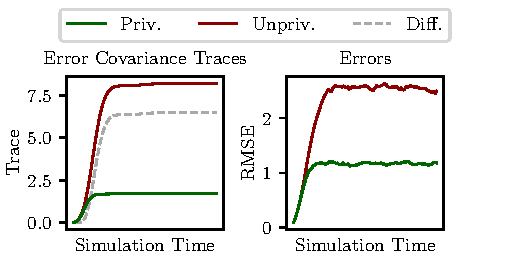
\includegraphics{pictures/single_level_bounded.pdf}
   \caption{Privileged estimation with bounded error covariance.}
   \label{fig:bounded}
\end{figure}

The second simulation considers an unobservable system where only the velocity is measured and has an unbounded error covariance as $k \rightarrow \infty$. It is given by
\begin{equation*}
   \mat{H}=
   \begin{bmatrix}
      0 & 1 & 0 & 0\\
      0 & 0 & 0 & 1
   \end{bmatrix}
\end{equation*}
and uses the same values for $\mat{R}$ and $\mat{Z}$ as given for the previous model. Figure \ref{fig:unbounded} shows the average error covariance traces and RMSE of estimation from 1000 runs using this model and capture how error covariance boundedness does not affect the privileged estimation scheme's properties.

\begin{figure}[htbp]
   \centering
   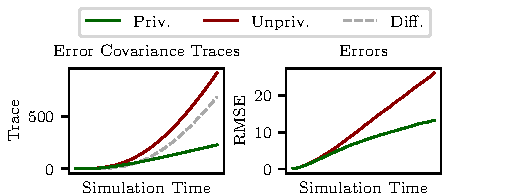
\includegraphics{pictures/single_level_unbounded.pdf}
   \caption{Privileged estimation with unbounded error covariance.}
   \label{fig:unbounded}
\end{figure}

Lastly, a simulation of multiple privilege levels was also performed using the bounded error covariance measurement model \eqref{eqn:bounded_sim_measurement_model} and using pseudorandom Gaussian samples such that $\mat{E}_1=20 \cdot \mat{I}$, $\mat{E}_2=14 \cdot \mat{I}$ and $\mat{E}_3=17 \cdot \mat{I}$. Note that the three matrices $\mat{E}_i$, $1 \leq i \leq 3$ satisfy \eqref{eqn:mult_covariance_restriction}. Figure \ref{fig:multiple} again shows the average traces and RMSE of estimation from 1000 runs and display the distinct difference in estimation error of the different privilege levels. Additionally, two special cases that bound all estimators are included, one holding all privilege level keys and another holding none.

\begin{figure}[htbp]
   \centering
   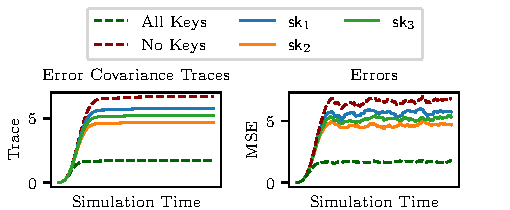
\includegraphics{pictures/multiple_level.pdf}
   \caption{Estimation with multiple privilege levels.}
   \label{fig:multiple}
\end{figure}

All of the included figures capture the difference in estimation error between the best possible estimators given the simulated processes (in terms of RMSE) and support the proposed security proof sketch given in section \ref{sec:scheme_security}.

% 
%  .d8888b.   .d88888b.  888b    888  .d8888b.  
% d88P  Y88b d88P" "Y88b 8888b   888 d88P  Y88b 
% 888    888 888     888 88888b  888 888    888 
% 888        888     888 888Y88b 888 888        
% 888        888     888 888 Y88b888 888        
% 888    888 888     888 888  Y88888 888    888 
% Y88b  d88P Y88b. .d88P 888   Y8888 Y88b  d88P 
%  "Y8888P"   "Y88888P"  888    Y888  "Y8888P"  
%                                               
%                                               
%                                               
% 

\section{Conclusion}\label{sec:conclusion}
In this work, we have presented the idea of a privileged estimation scheme and given a formal cryptographic definition for its security. A concrete scheme was provided with a proof sketch for meeting this notion and an intuitive extension to multiple privileged levels was discussed. The benefits of controlling estimation accuracy on a per-party basis have countless applications from privatized localization hardware to subscription-based data access and a suitable simulation demonstrating a simple use-case for object tracking has been presented. Possible future work on the topic includes reducing the requirement in \eqref{eqn:mult_covariance_restriction} to make multiple privilege levels more applicable, achieving formal security for broader model requirements, and implementing a privileged estimation scheme on hardware to demonstrate the real-time capability of the method.

% conference papers do not normally have an appendix

% use section* for acknowledgment
%\section*{Acknowledgment}

% Bibliography
\bibliographystyle{IEEEtran}
\bibliography{BibTeX/PrivilegedEstimation}

% that's all folks
\end{document}


